\documentclass[twoside,twocolumn]{article}

\usepackage{blindtext} 
\usepackage{graphicx}
\usepackage[sc]{mathpazo} 
\usepackage[T1]{fontenc} 
\linespread{1.05} 
\usepackage{microtype} 


\usepackage[english]{babel} 


\usepackage[hmarginratio=1:1,top=32mm,columnsep=20pt]{geometry} 
\usepackage[hang, small,labelfont=bf,up,textfont=it,up]{caption} 
\usepackage{booktabs} 


\usepackage{lettrine} 


\usepackage{enumitem} 
\setlist[itemize]{noitemsep} 


\usepackage{abstract} 
\renewcommand{\abstractnamefont}{\normalfont\bfseries} 
\renewcommand{\abstracttextfont}{\normalfont\small\itshape} 


\usepackage{titlesec} 
\renewcommand\thesection{\Roman{section}} % 
\renewcommand\thesubsection{\roman{subsection}} 
\titleformat{\section}[block]{\large\scshape\centering}{\thesection.}{1em}{} 
\titleformat{\subsection}[block]{\large}{\thesubsection.}{1em}{} 


\usepackage{fancyhdr} 
\pagestyle{fancy} 
\fancyhead{} 
\fancyfoot{} 
\fancyhead[C]{Inmon vs Kimball $\bullet$ Octubre 2019 $\bullet$ } 
\fancyfoot[RO,LE]{\thepage} 


\usepackage{titling} 


\usepackage{hyperref} 


%----------------------------------------------------------------------------------------
%	TILULOS
%----------------------------------------------------------------------------------------


\setlength{\droptitle}{-4\baselineskip} 

\pretitle{\begin{center}\Huge\bfseries} 
\posttitle{\end{center}} 
\title{Inmon vs Kimball} 
\author{Jose Condori Choquecota\\
}
\date{Octubre 2019} 
\renewcommand{\maketitlehookd}{

\begin{abstract}
\noindent 
Los métodos Inmon y Kimball se pueden usar para diseñar con éxito almacenes de datos. De hecho, varias empresas utilizan una combinación de ambos enfoques (llamado modelo híbrido).En el modelo híbrido, el método Inmon se usa para formar un almacén de datos integrado. Mientras que, se sigue el enfoque de Kimball para desarrollar marts de datos utilizando el esquema de estrella.
No es posible afirmar qué enfoque es mejor ya que ambos métodos tienen sus ventajas y desventajas, y ambos funcionan bien en diferentes situaciones. El diseñador del almacén de datos tiene que elegir un método dependiendo de los diversos factores discutidos en este artículo.
Por último, para que cualquier método sea efectivo, tiene que estar bien pensado, explorado en profundidad y desarrollado para satisfacer los requisitos de informes de inteligencia empresarial de su empresa.


\end{abstract}


\begin{abstract}
\noindent 
The Inmon and Kimball methods can be used to successfully design data stores. In fact, several companies use a combination of both approaches (called a hybrid model).In the hybrid model, the Inmon method is used to form an integrated data warehouse. Meanwhile, Kimball's approach to developing data marts using the star scheme is followed.
It is not possible to state which approach is better since both methods have their advantages and disadvantages, and both work well in different situations. The data warehouse designer has to choose a method depending on the various factors discussed in this article.
Finally, for any method to be effective, it has to be well thought out, explored in depth and developed to meet the business intelligence reporting requirements of your company.
\end{abstract}
}

%----------------------------------------------------------------------------------------

\begin{document}

% Print the title
\maketitle

%----------------------------------------------------------------------------------------
%	INTRODUCCION
%----------------------------------------------------------------------------------------

\section{Introduccion}
\lettrine[nindent=0em,lines=3]{E}stamos viviendo en la era de una revolución de datos, y más corporaciones se están dando cuenta de que para liderar, o en algunos casos, para sobrevivir, necesitan aprovechar su riqueza de datos de manera efectiva. El almacén de datos, debido a su propuesta única como el repositorio empresarial integrado de datos, está jugando un papel aún más importante en esta situación. Actualmente se practican dos estilos de arquitectura prominentes para construir un almacén de datos: la arquitectura Inmon y la arquitectura Kimball. Este artículo intenta comparar y contrastar los pros y los contras de cada estilo de arquitectura y recomendar qué estilo seguir basándose en ciertos factores.




%----------------------------------------------------------------------------------------
%	Objetivos
%----------------------------------------------------------------------------------------


\section{Objetivos}

\begin{itemize}

\item \textbf{ Inmon y Kimball}
\\
\item Entender la importancia del Data Ware House en las empresas, organizaciones, entidades,intitucíones, etc.
\item Desarrollar los antecedentes de la metodologia decrita por William H. Inmon y Ralph Kimball.
\item Compartivo de las metodologias descritas por William H. Inmon y Ralph Kimball.
\\



\end{itemize}


%----------------------------------------------------------------------------------------
%	Marco teorico
%----------------------------------------------------------------------------------------


\section{Marco teorico}
\begin{enumerate}
\item \textbf{E}l enfoque de Inmon para construir un almacén de datos comienza con el modelo de datos corporativos. Este modelo identifica las áreas temáticas clave y, lo que es más importante, las entidades clave con las que opera y se preocupa la empresa, como el cliente, el producto, el proveedor, etc. A partir de este modelo, se crea un modelo lógico detallado para cada entidad principal. Por ejemplo, se creará un modelo lógico para el Cliente con todos los detalles relacionados con esa entidad. Podría haber diez entidades diferentes bajo Cliente. Todos los detalles, incluidas las claves comerciales, los atributos, las dependencias, la participación y las relaciones, se capturarán en el modelo lógico detallado. El punto clave aquí es que la estructura de la entidad está construida en forma normalizada. La redundancia de datos se evita tanto como sea posible. Esto conduce a una identificación clara de los conceptos comerciales y evita anomalías en la actualización de datos. El siguiente paso es construir el modelo físico. La implementación física del almacén de datos también está normalizada. Esto es lo que Inmon llama como un 'almacén de datos', y aquí es donde se gestiona la versión única de la verdad para la empresa. Este modelo normalizado hace que cargar los datos sea menos complejo, pero usar esta estructura para realizar consultas es difícil ya que involucra muchas tablas y uniones. Entonces, Inmon sugiere construir data marts específicos para los departamentos. Los mercados de datos se diseñarán específicamente para Finanzas, Ventas, etc., y los mercados de datos pueden tener datos desnormalizados para ayudar con los informes (Breslin, 2004). Todos los datos que ingresan al almacén de datos están integrados, y el almacén de datos es la única fuente de datos para los diferentes mercados de datos. Esto garantiza que la integridad y la consistencia de los datos se mantengan intactos en toda la organización.\\ \\
Los activos intangibles se han posicionado como un valor base para asegurar el crecimiento de las empresas[1].

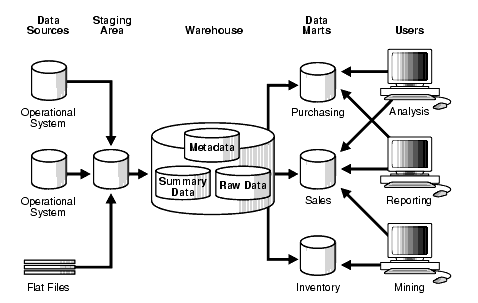
\includegraphics[width=7cm]{Imagenes/1.PNG}
\textbf{ {\small  Fig: Fuente: Stanford. 2003. "Conceptos de almacenamiento de datos"}}
\\ \\



\textbf{Las ventajas clave del enfoque de Inmon son:}
\\
\begin{itemize}
\item El almacén de datos realmente sirve como la única fuente de verdad para la empresa, ya que es la única fuente para los mercados de datos y todos los datos en el almacén de datos están integrados.
\item Se evitan las anomalías en la actualización de datos debido a la baja redundancia. Esto hace que el proceso ETL sea más fácil y menos propenso a fallas.
\item Los procesos comerciales se pueden entender fácilmente, ya que el modelo lógico representa las entidades comerciales detalladas.
\item Muy flexible: a medida que cambian los requisitos comerciales o cambian los datos de origen, es fácil actualizar el almacén de datos ya que una cosa está en un solo lugar.
\item Puede manejar diversas necesidades de informes en toda la empresa.
\end{itemize}

\textbf{Estas son algunas de las desventajas del método Inmon:}
\begin{itemize}
\item El modelo y la implementación pueden volverse complejos con el tiempo, ya que implica más tablas y combinaciones.
\item Necesita recursos expertos en modelado de datos y en el negocio mismo. Este tipo de recursos puede ser difícil de encontrar y a menudo son caros.
\item La configuración inicial y la entrega tomarán más tiempo, y la gerencia debe ser consciente de esto.
\item Se necesita más trabajo ETL ya que los data marts se crean desde el almacén de datos
\item Se necesita un equipo bastante grande de especialistas para administrar con éxito el medio ambiente (Breslin, 2004).
\end{itemize}


   
\textbf El enfoque de Kimball \\ 


El enfoque de Kimball para construir el almacén de datos comienza con la identificación de los procesos comerciales clave y las preguntas comerciales clave que el almacén de datos debe responder. Las fuentes clave (sistemas operativos) de datos para el almacén de datos se analizan y documentan. El software ETL se utiliza para llevar datos de todas las diferentes fuentes y cargarlos en un área de preparación. A partir de aquí, los datos se cargan en un modelo dimensional. Aquí viene la diferencia clave: el modelo propuesto por Kimball para el almacenamiento de datos, el modelo dimensional, no está normalizado. El concepto fundamental del modelado dimensional es el esquema estelar. En el esquema de estrella, generalmente hay una tabla de hechos rodeada de muchas dimensiones. La tabla de hechos tiene todas las medidas que son relevantes para el área temática, y también tiene las claves externas de las diferentes dimensiones que rodean el hecho. Las dimensiones se desnormalizan por completo para que el usuario pueda profundizar y profundizar sin unirse a otra tabla. Se crearán múltiples esquemas en estrella para satisfacer diferentes requisitos de informes. Entonces, ¿cómo se logra la integración en el modelo dimensional? Aquí, Kimball propone el concepto de 'dimensiones conformadas'. Las dimensiones clave, como el cliente y el producto, que se comparten entre los diferentes hechos se construirán una vez y se utilizarán en todos los hechos (Kimball et al. 2013). Esto asegura que una cosa o concepto se use de la misma manera en todos los hechos. Otro artefacto clave del modelo Kimball es la 'matriz de bus empresarial'. Este es el documento donde los diferentes hechos se enumeran verticalmente y las dimensiones conformadas se enumeran horizontalmente. Siempre que las dimensiones juegan un papel clave extranjero en el hecho, está marcado en el documento. Esto sirve como un documento de anclaje que muestra cómo se construyen los esquemas en estrella y qué queda por construir en el almacén de datos. La Figura 1.3 muestra una arquitectura típica de almacén de datos de Kimball.
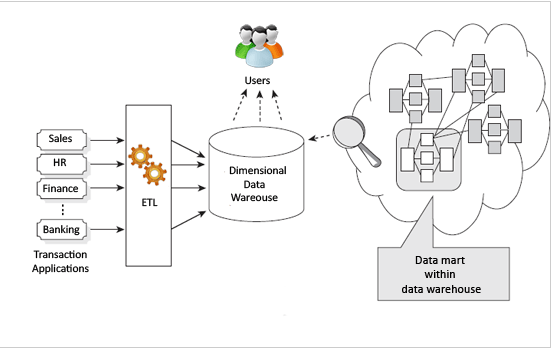
\includegraphics[width=7cm]{Imagenes/2.png}
\textbf{ {\small  Fig: Fuente: Zentut. 2016. "Ralph Kimball Data Warehouse Architecture}}
\\ \\

\begin{enumerate}
\item[1.1] Estas son algunas de las ventajas del método Kimball: \\ 
\item Rápido de configurar y construir, y la primera fase del proyecto de almacenamiento de datos se entregará rápidamente.
\item El esquema de estrella puede ser fácilmente entendido por los usuarios comerciales y es fácil de usar para generar informes. La mayoría de las herramientas de BI funcionan bien con el esquema en estrella.
\item La huella del entorno de almacenamiento de datos es pequeña; ocupa menos espacio en la base de datos y facilita la administración del sistema.
\item El rendimiento del modelo de esquema en estrella es muy bueno. El motor de la base de datos realizará una 'unión en estrella' donde se creará un producto cartesiano utilizando todos los valores de dimensión y la tabla de hechos se consultará finalmente para las filas selectivas. Esto se sabe que es una operación de base de datos muy efectiva.
\item Un pequeño equipo de desarrolladores y arquitectos es suficiente para mantener el almacenamiento de datos funcionando de manera efectiva (Breslin, 2004).
\item Funciona realmente bien para las métricas en función del departamento y el seguimiento de KPI, ya que los data marts están orientados a la elaboración de informes por departamento o por proceso empresarial.
\item La obtención de detalles, donde una herramienta de BI atraviesa múltiples esquemas en estrella para generar un informe, se puede lograr con éxito utilizando dimensiones conformadas.


\item[1.2] Estas son algunas de las desventajas del método Kimball: \\ 
\item La esencia de la 'única fuente de verdad' se pierde, ya que los datos no se integran completamente antes de satisfacer las necesidades de informes.
\item Los datos redundantes pueden causar anomalías en la actualización de datos con el tiempo.
\item Agregar columnas a la tabla de hechos puede causar problemas de rendimiento. Esto se debe a que las tablas de hechos están diseñadas para ser muy profundas. Si se van a agregar nuevas columnas, el tamaño de la tabla de hechos se vuelve mucho más grande y no funcionará bien. Esto hace que el modelo dimensional sea difícil de cambiar a medida que cambian los requisitos comerciales.
\item No se pueden manejar todas las necesidades de informes de la empresa porque el modelo está orientado hacia los procesos comerciales en lugar de la empresa en su conjunto.
\item La integración de datos heredados en el almacén de datos puede ser un proceso complejo.




\end{enumerate}
    
\end{enumerate}





%----------------------------------------------------------------------------------------
%	Ejemplo
%----------------------------------------------------------------------------------------



%----------------------------------------------------------------------------------------
%	Análisis
%----------------------------------------------------------------------------------------


\section{Análisis}
Ahora que hemos visto los pros y los contras de los enfoques de Kimball e Inmon, surge una pregunta. ¿Qué enfoque debe usarse cuando? Los arquitectos del almacén de datos enfrentan esta pregunta cada vez que comienzan a construir un almacén de datos. Estos son los factores decisivos que pueden ayudar a un arquitecto a elegir entre los dos:\\
\begin{itemize}
 \item Requisitos de informes : si los requisitos de informes son estratégicos y se necesitan informes integrados para toda la empresa, entonces Inmon funciona mejor. Si los requisitos de presentación de informes son tácticos y orientados al proceso de negocio / equipo, entonces Kimball funciona mejor.\\


 \item Proyecto de urgencia : si la organización tiene tiempo suficiente para esperar la primera entrega del almacén de datos (por ejemplo, de 4 a 9 meses), se puede seguir el enfoque de Inmon. Si hay muy poco tiempo para que el almacén de datos esté en funcionamiento (por ejemplo, de 2 a 3 meses), entonces el enfoque de Kimball es el mejor (Breslin, 2004).\\
 \item Plan de dotación de personal futuro : si la empresa puede permitirse tener un equipo de especialistas de gran tamaño para mantener el almacén de datos, entonces se puede seguir el método Inmon. Si el plan futuro para el equipo es ser delgado, entonces Kimball es más adecuado.
 \item Frecuencia de cambios : si se espera que los requisitos de informes cambien más rápidamente y se sepa que los sistemas de origen son volátiles, entonces el enfoque de Inmon funciona mejor, ya que es más flexible. Si los requisitos y los sistemas fuente son relativamente estables, se puede utilizar el método Kimball.\\
 \item Cultura de la organización : si los patrocinadores del almacén de datos y los gerentes de la empresa entienden la propuesta de valor del almacén de datos y están dispuestos a aceptar un valor duradero de la inversión del almacén de datos, el enfoque de Inmon es mejor. Si los patrocinadores no se preocupan por los conceptos pero quieren una solución para mejorar en la presentación de informes, entonces el enfoque de Kimball es suficiente.\\

\end{itemize} 



%----------------------------------------------------------------------------------------
%	CONCLUSIONES
%----------------------------------------------------------------------------------------

\section{Conclusiones}
\begin{itemize}	
 \item Se ha demostrado que tanto el enfoque de Inmon como el de Kimball funcionan para entregar con éxito almacenes de datos. Incluso hay organizaciones donde se ha implementado una combinación de ambos ('modelo híbrido'). En un modelo híbrido, el almacén de datos se construye utilizando el modelo Inmon, y además del almacén de datos integrado, los almacenes de datos orientados a procesos de negocio se construyen utilizando el esquema en estrella para la presentación de informes. No podemos generalizar y decir que un enfoque es mejor que el otro; Ambos tienen sus ventajas y desventajas, y ambos funcionan bien en diferentes escenarios. El arquitecto tiene que seleccionar un enfoque para el almacén de datos en función de los diferentes factores; Se identificaron algunas claves en este documento. Finalmente, para que cualquier enfoque sea exitoso, debe ser cuidadosamente pensado, discutido en detalle,
\\


\end{itemize} 



%----------------------------------------------------------------------------------------
%	BIBLIOGRAFIA
%----------------------------------------------------------------------------------------


\begin{thebibliography}{99} 

\bibitem[1]{}
\newblock Breslin, Mary. 2004. "Data Warehousing Battle of the Giants: Comparing the Basics of the Kimball and Inmon Models" Business Intelligence Journal, invierno de 2004. Consultado el 22 de mayo de 2016.

\bibitem[2]{}
\newblock Inmon, WH  Construyendo el Data Warehouse, cuarta edición . John Wiley y Sons., 2005.

\bibitem[3]{}
\newblock Marakas, George M.  Almacenamiento moderno de datos, minería y visualización . Prentice Hall, 2003.

\bibitem[4]{}
\newblock Inmon, WH 2010. “UNA CUENTA DE DOS ARQUITECTURAS” InmonCif.com. Consultado el 23 de mayo de 2016.InmonCif . com . Consultado el 23 de mayo de 2016.
\bibitem[5]{}
\newblock Kimball, Ralph y Margy Ross. The Data Warehouse Toolkit: The Definitive Guide to Dimensional Modeling, Third Edition . John Wiley y Sons. 2013. Libros 24x7.
\bibitem[6]{}
\newblock Zentut 2016. "Arquitectura del almacén de datos Ralph Kimball" Zentut.com. Consultado el 25 de mayo de 2016.  http://www.zentut.com/data-warehouse/ralph-kimball-data-warehouse-architecture/Zentut . com . Consultado el 25 de mayo de 2016. 




\end{thebibliography}


%----------------------------------------------------------------------------------------


\end{document}
